
%% bare_jrnl.tex
%% V1.3
%% 2007/01/11
%% by Michael Shell
%% see http://www.michaelshell.org/
%% for current contact information.
%%
%% This is a skeleton file demonstrating the use of IEEEtran.cls
%% (requires IEEEtran.cls version 1.7 or later) with an IEEE journal paper.
%%
%% Support sites:
%% http://www.michaelshell.org/tex/ieeetran/
%% http://www.ctan.org/tex-archive/macros/latex/contrib/IEEEtran/
%% and
%% http://www.ieee.org/



% *** Authors should verify (and, if needed, correct) their LaTeX system  ***
% *** with the testflow diagnostic prior to trusting their LaTeX platform ***
% *** with production work. IEEE's font choices can trigger bugs that do  ***
% *** not appear when using other class files.                            ***
% The testflow support page is at:
% http://www.michaelshell.org/tex/testflow/


%%*************************************************************************
%% Legal Notice:
%% This code is offered as-is without any warranty either expressed or
%% implied; without even the implied warranty of MERCHANTABILITY or
%% FITNESS FOR A PARTICULAR PURPOSE! 
%% User assumes all risk.
%% In no event shall IEEE or any contributor to this code be liable for
%% any damages or losses, including, but not limited to, incidental,
%% consequential, or any other damages, resulting from the use or misuse
%% of any information contained here.
%%
%% All comments are the opinions of their respective authors and are not
%% necessarily endorsed by the IEEE.
%%
%% This work is distributed under the LaTeX Project Public License (LPPL)
%% ( http://www.latex-project.org/ ) version 1.3, and may be freely used,
%% distributed and modified. A copy of the LPPL, version 1.3, is included
%% in the base LaTeX documentation of all distributions of LaTeX released
%% 2003/12/01 or later.
%% Retain all contribution notices and credits.
%% ** Modified files should be clearly indicated as such, including  **
%% ** renaming them and changing author support contact information. **
%%
%% File list of work: IEEEtran.cls, IEEEtran_HOWTO.pdf, bare_adv.tex,
%%                    bare_conf.tex, bare_jrnl.tex, bare_jrnl_compsoc.tex
%%*************************************************************************

% Note that the a4paper option is mainly intended so that authors in
% countries using A4 can easily print to A4 and see how their papers will
% look in print - the typesetting of the document will not typically be
% affected with changes in paper size (but the bottom and side margins will).
% Use the testflow package mentioned above to verify correct handling of
% both paper sizes by the user's LaTeX system.
%
% Also note that the "draftcls" or "draftclsnofoot", not "draft", option
% should be used if it is desired that the figures are to be displayed in
% draft mode.
%
\documentclass[11pt,journal]{IEEEtran}
\usepackage{blindtext}
\usepackage{graphicx}
\usepackage{subcaption}
\usepackage{gensymb}

\renewcommand{\baselinestretch}{1.5}

% Some very useful LaTeX packages include:
% (uncomment the ones you want to load)


% *** MISC UTILITY PACKAGES ***
%
%\usepackage{ifpdf}
% Heiko Oberdiek's ifpdf.sty is very useful if you need conditional
% compilation based on whether the output is pdf or dvi.
% usage:
% \ifpdf
%   % pdf code
% \else
%   % dvi code
% \fi
% The latest version of ifpdf.sty can be obtained from:
% http://www.ctan.org/tex-archive/macros/latex/contrib/oberdiek/
% Also, note that IEEEtran.cls V1.7 and later provides a builtin
% \ifCLASSINFOpdf conditional that works the same way.
% When switching from latex to pdflatex and vice-versa, the compiler may
% have to be run twice to clear warning/error messages.






% *** CITATION PACKAGES ***
%
%\usepackage{cite}
% cite.sty was written by Donald Arseneau
% V1.6 and later of IEEEtran pre-defines the format of the cite.sty package
% \cite{} output to follow that of IEEE. Loading the cite package will
% result in citation numbers being automatically sorted and properly
% "compressed/ranged". e.g., [1], [9], [2], [7], [5], [6] without using
% cite.sty will become [1], [2], [5]--[7], [9] using cite.sty. cite.sty's
% \cite will automatically add leading space, if needed. Use cite.sty's
% noadjust option (cite.sty V3.8 and later) if you want to turn this off.
% cite.sty is already installed on most LaTeX systems. Be sure and use
% version 4.0 (2003-05-27) and later if using hyperref.sty. cite.sty does
% not currently provide for hyperlinked citations.
% The latest version can be obtained at:
% http://www.ctan.org/tex-archive/macros/latex/contrib/cite/
% The documentation is contained in the cite.sty file itself.






% *** GRAPHICS RELATED PACKAGES ***
%
\ifCLASSINFOpdf
  % \usepackage[pdftex]{graphicx}
  % declare the path(s) where your graphic files are
  % \graphicspath{{../pdf/}{../jpeg/}}
  % and their extensions so you won't have to specify these with
  % every instance of \includegraphics
  % \DeclareGraphicsExtensions{.pdf,.jpeg,.png}
\else
  % or other class option (dvipsone, dvipdf, if not using dvips). graphicx
  % will default to the driver specified in the system graphics.cfg if no
  % driver is specified.
  % \usepackage[dvips]{graphicx}
  % declare the path(s) where your graphic files are
  % \graphicspath{{../eps/}}
  % and their extensions so you won't have to specify these with
  % every instance of \includegraphics
  % \DeclareGraphicsExtensions{.eps}
\fi
% graphicx was written by David Carlisle and Sebastian Rahtz. It is
% required if you want graphics, photos, etc. graphicx.sty is already
% installed on most LaTeX systems. The latest version and documentation can
% be obtained at: 
% http://www.ctan.org/tex-archive/macros/latex/required/graphics/
% Another good source of documentation is "Using Imported Graphics in
% LaTeX2e" by Keith Reckdahl which can be found as epslatex.ps or
% epslatex.pdf at: http://www.ctan.org/tex-archive/info/
%
% latex, and pdflatex in dvi mode, support graphics in encapsulated
% postscript (.eps) format. pdflatex in pdf mode supports graphics
% in .pdf, .jpeg, .png and .mps (metapost) formats. Users should ensure
% that all non-photo figures use a vector format (.eps, .pdf, .mps) and
% not a bitmapped formats (.jpeg, .png). IEEE frowns on bitmapped formats
% which can result in "jaggedy"/blurry rendering of lines and letters as
% well as large increases in file sizes.
%
% You can find documentation about the pdfTeX application at:
% http://www.tug.org/applications/pdftex





% *** MATH PACKAGES ***
%
%\usepackage[cmex10]{amsmath}
% A popular package from the American Mathematical Society that provides
% many useful and powerful commands for dealing with mathematics. If using
% it, be sure to load this package with the cmex10 option to ensure that
% only type 1 fonts will utilized at all point sizes. Without this option,
% it is possible that some math symbols, particularly those within
% footnotes, will be rendered in bitmap form which will result in a
% document that can not be IEEE Xplore compliant!
%
% Also, note that the amsmath package sets \interdisplaylinepenalty to 10000
% thus preventing page breaks from occurring within multiline equations. Use:
%\interdisplaylinepenalty=2500
% after loading amsmath to restore such page breaks as IEEEtran.cls normally
% does. amsmath.sty is already installed on most LaTeX systems. The latest
% version and documentation can be obtained at:
% http://www.ctan.org/tex-archive/macros/latex/required/amslatex/math/





% *** SPECIALIZED LIST PACKAGES ***
%
%\usepackage{algorithmic}
% algorithmic.sty was written by Peter Williams and Rogerio Brito.
% This package provides an algorithmic environment fo describing algorithms.
% You can use the algorithmic environment in-text or within a figure
% environment to provide for a floating algorithm. Do NOT use the algorithm
% floating environment provided by algorithm.sty (by the same authors) or
% algorithm2e.sty (by Christophe Fiorio) as IEEE does not use dedicated
% algorithm float types and packages that provide these will not provide
% correct IEEE style captions. The latest version and documentation of
% algorithmic.sty can be obtained at:
% http://www.ctan.org/tex-archive/macros/latex/contrib/algorithms/
% There is also a support site at:
% http://algorithms.berlios.de/index.html
% Also of interest may be the (relatively newer and more customizable)
% algorithmicx.sty package by Szasz Janos:
% http://www.ctan.org/tex-archive/macros/latex/contrib/algorithmicx/




% *** ALIGNMENT PACKAGES ***
%
%\usepackage{array}
% Frank Mittelbach's and David Carlisle's array.sty patches and improves
% the standard LaTeX2e array and tabular environments to provide better
% appearance and additional user controls. As the default LaTeX2e table
% generation code is lacking to the point of almost being broken with
% respect to the quality of the end results, all users are strongly
% advised to use an enhanced (at the very least that provided by array.sty)
% set of table tools. array.sty is already installed on most systems. The
% latest version and documentation can be obtained at:
% http://www.ctan.org/tex-archive/macros/latex/required/tools/


%\usepackage{mdwmath}
%\usepackage{mdwtab}
% Also highly recommended is Mark Wooding's extremely powerful MDW tools,
% especially mdwmath.sty and mdwtab.sty which are used to format equations
% and tables, respectively. The MDWtools set is already installed on most
% LaTeX systems. The lastest version and documentation is available at:
% http://www.ctan.org/tex-archive/macros/latex/contrib/mdwtools/


% IEEEtran contains the IEEEeqnarray family of commands that can be used to
% generate multiline equations as well as matrices, tables, etc., of high
% quality.


%\usepackage{eqparbox}
% Also of notable interest is Scott Pakin's eqparbox package for creating
% (automatically sized) equal width boxes - aka "natural width parboxes".
% Available at:
% http://www.ctan.org/tex-archive/macros/latex/contrib/eqparbox/





% *** SUBFIGURE PACKAGES ***
%\usepackage[tight,footnotesize]{subfigure}
% subfigure.sty was written by Steven Douglas Cochran. This package makes it
% easy to put subfigures in your figures. e.g., "Figure 1a and 1b". For IEEE
% work, it is a good idea to load it with the tight package option to reduce
% the amount of white space around the subfigures. subfigure.sty is already
% installed on most LaTeX systems. The latest version and documentation can
% be obtained at:
% http://www.ctan.org/tex-archive/obsolete/macros/latex/contrib/subfigure/
% subfigure.sty has been superceeded by subfig.sty.



%\usepackage[caption=false]{caption}
%\usepackage[font=footnotesize]{subfig}
% subfig.sty, also written by Steven Douglas Cochran, is the modern
% replacement for subfigure.sty. However, subfig.sty requires and
% automatically loads Axel Sommerfeldt's caption.sty which will override
% IEEEtran.cls handling of captions and this will result in nonIEEE style
% figure/table captions. To prevent this problem, be sure and preload
% caption.sty with its "caption=false" package option. This is will preserve
% IEEEtran.cls handing of captions. Version 1.3 (2005/06/28) and later 
% (recommended due to many improvements over 1.2) of subfig.sty supports
% the caption=false option directly:
%\usepackage[caption=false,font=footnotesize]{subfig}
%
% The latest version and documentation can be obtained at:
% http://www.ctan.org/tex-archive/macros/latex/contrib/subfig/
% The latest version and documentation of caption.sty can be obtained at:
% http://www.ctan.org/tex-archive/macros/latex/contrib/caption/




% *** FLOAT PACKAGES ***
%
%\usepackage{fixltx2e}
% fixltx2e, the successor to the earlier fix2col.sty, was written by
% Frank Mittelbach and David Carlisle. This package corrects a few problems
% in the LaTeX2e kernel, the most notable of which is that in current
% LaTeX2e releases, the ordering of single and double column floats is not
% guaranteed to be preserved. Thus, an unpatched LaTeX2e can allow a
% single column figure to be placed prior to an earlier double column
% figure. The latest version and documentation can be found at:
% http://www.ctan.org/tex-archive/macros/latex/base/



%\usepackage{stfloats}
% stfloats.sty was written by Sigitas Tolusis. This package gives LaTeX2e
% the ability to do double column floats at the bottom of the page as well
% as the top. (e.g., "\begin{figure*}[!b]" is not normally possible in
% LaTeX2e). It also provides a command:
%\fnbelowfloat
% to enable the placement of footnotes below bottom floats (the standard
% LaTeX2e kernel puts them above bottom floats). This is an invasive package
% which rewrites many portions of the LaTeX2e float routines. It may not work
% with other packages that modify the LaTeX2e float routines. The latest
% version and documentation can be obtained at:
% http://www.ctan.org/tex-archive/macros/latex/contrib/sttools/
% Documentation is contained in the stfloats.sty comments as well as in the
% presfull.pdf file. Do not use the stfloats baselinefloat ability as IEEE
% does not allow \baselineskip to stretch. Authors submitting work to the
% IEEE should note that IEEE rarely uses double column equations and
% that authors should try to avoid such use. Do not be tempted to use the
% cuted.sty or midfloat.sty packages (also by Sigitas Tolusis) as IEEE does
% not format its papers in such ways.


%\ifCLASSOPTIONcaptionsoff
%  \usepackage[nomarkers]{endfloat}
% \let\MYoriglatexcaption\caption
% \renewcommand{\caption}[2][\relax]{\MYoriglatexcaption[#2]{#2}}
%\fi
% endfloat.sty was written by James Darrell McCauley and Jeff Goldberg.
% This package may be useful when used in conjunction with IEEEtran.cls'
% captionsoff option. Some IEEE journals/societies require that submissions
% have lists of figures/tables at the end of the paper and that
% figures/tables without any captions are placed on a page by themselves at
% the end of the document. If needed, the draftcls IEEEtran class option or
% \CLASSINPUTbaselinestretch interface can be used to increase the line
% spacing as well. Be sure and use the nomarkers option of endfloat to
% prevent endfloat from "marking" where the figures would have been placed
% in the text. The two hack lines of code above are a slight modification of
% that suggested by in the endfloat docs (section 8.3.1) to ensure that
% the full captions always appear in the list of figures/tables - even if
% the user used the short optional argument of \caption[]{}.
% IEEE papers do not typically make use of \caption[]'s optional argument,
% so this should not be an issue. A similar trick can be used to disable
% captions of packages such as subfig.sty that lack options to turn off
% the subcaptions:
% For subfig.sty:
% \let\MYorigsubfloat\subfloat
% \renewcommand{\subfloat}[2][\relax]{\MYorigsubfloat[]{#2}}
% For subfigure.sty:
% \let\MYorigsubfigure\subfigure
% \renewcommand{\subfigure}[2][\relax]{\MYorigsubfigure[]{#2}}
% However, the above trick will not work if both optional arguments of
% the \subfloat/subfig command are used. Furthermore, there needs to be a
% description of each subfigure *somewhere* and endfloat does not add
% subfigure captions to its list of figures. Thus, the best approach is to
% avoid the use of subfigure captions (many IEEE journals avoid them anyway)
% and instead reference/explain all the subfigures within the main caption.
% The latest version of endfloat.sty and its documentation can obtained at:
% http://www.ctan.org/tex-archive/macros/latex/contrib/endfloat/
%
% The IEEEtran \ifCLASSOPTIONcaptionsoff conditional can also be used
% later in the document, say, to conditionally put the References on a 
% page by themselves.


% *** PDF, URL AND HYPERLINK PACKAGES ***
%
%\usepackage{url}
% url.sty was written by Donald Arseneau. It provides better support for
% handling and breaking URLs. url.sty is already installed on most LaTeX
% systems. The latest version can be obtained at:
% http://www.ctan.org/tex-archive/macros/latex/contrib/misc/
% Read the url.sty source comments for usage information. Basically,
% \url{my_url_here}.





% *** Do not adjust lengths that control margins, column widths, etc. ***
% *** Do not use packages that alter fonts (such as pslatex).         ***
% There should be no need to do such things with IEEEtran.cls V1.6 and later.
% (Unless specifically asked to do so by the journal or conference you plan
% to submit to, of course. )


% correct bad hyphenation here
\hyphenation{op-tical net-works semi-conduc-tor}


\begin{document}
%
% paper title
% can udse linebreaks \\ within to get better formatting as desired
\title{Design of an Autonomous Racing Vehicle}
%
%
% author names and IEEE memberships
% note positions of commas and nonbreaking spaces ( ~ ) LaTeX will not break
% a structure at a ~ so this keeps an author's name from being broken across
% two lines.
% use \thanks{} to gain access to the first footnote area
% a separate \thanks must be used for each paragraph as LaTeX2e's \thanks
% was not built to handle multiple paragraphs
%

\author{Oluwatoni~Ogunmade, Jack~Xu, Tsugumi~Murata, Adrian~Malanaran,  Angela~Gu, Brian~Tran, Andrew~Jin, Waleed~Ahmed, Brian~Kibazohi, Jun-Ha~Jung
        % <-this % stops a space
\thanks{Contributors are from the Departments of Mathematics and Engineering at the University of Waterloo and the Department of Engineering at McMaster University.}}

% note the % following the last \IEEEmembership and also \thanks - 
% these prevent an unwanted space from occurring between the last author name
% and the end of the author line. i.e., if you had this:
% 
% \author{....lastname \thanks{...} \thanks{...} }
%                     ^------------^------------^----Do not want these spaces!
%
% a space would be appended to the last name and could cause every name on that
% line to be shifted left slightly. This is one of those "LaTeX things". For
% instance, "\textbf{A} \textbf{B}" will typeset as "A B" not "AB". To get
% "AB" then you have to do: "\textbf{A}\textbf{B}"
% \thanks is no different in this regard, so shield the last } of each \thanks
% that ends a line with a % and do not let a space in before the next \thanks.
% Spaces after \IEEEmembership other than the last one are OK (and needed) as
% you are supposed to have spaces between the names. For what it is worth,
% this is a minor point as most people would not even notice if the said evil
% space somehow managed to creep in.



% The paper headers
\markboth{International Autonomous Robot Racing Competition - University of Waterloo Submission}%
{Shell \MakeLowercase{\textit{et al.}}: Bare Demo of IEEEtran.cls for Journals}
% The only time the second header will appear is for the odd numbered pages
% after the title page when using the twoside option.
% 
% *** Note that you probably will NOT want to include the author's ***
% *** name in the headers of peer review papers.                   ***
% You can use \ifCLASSOPTIONpeerreview for conditional compilation here if
% you desire.




% If you want to put a publisher's ID mark on the page you can do it like
% this:
%\IEEEpubid{0000--0000/00\$00.00~\copyright~2007 IEEE}
% Remember, if you use this you must call \IEEEpubidadjcol in the second
% column for its text to clear the IEEEpubid mark.



% use for special paper notices
%\IEEEspecialpapernotice{(Invited Paper)}




% make the title area
\maketitle


\begin{abstract}

This technical report describes the University of Waterloo's team approach to the International Autonomous Robot Racing Competition(IARRC). We developed a system capable of real-time autonomous driving utilizing off-the-shelf parts including three cameras, an Inertial Measurement Unit(IMU), a quadrature encoder and a Hokuyo planar Lidar. The vehicle is a modified 1:10th scale Traxxas RC car with electronics to support battery monitoring, power distribution, remote control and emergency stopping. A robust and modular aluminum superstructure was built as a retrofit system for the vehicle, to provide a reliable and accessible platform for developing autonomous cruising system. A cutting edge neural net based traffic light detection system was added to improve robustness. A new path planner was designed relying on a Random-exploring Random Tree(RRT) planner, a Model Predictive Controller(MPC) for longer range planning and a trajectory rollout algorithm for short range evasive maneuvers.

In this paper we will focus on innovations in our overall approach by highlighting our computer vision, system architecture, software development practices, path planning and controls.


\end{abstract}
% IEEEtran.cls defaults to using nonbold math in the Abstract.
% This preserves the distinction between vectors and scalars. However,
% if the journal you are submitting to favors bold math in the abstract,
% then you can use LaTeX's standard command \boldmath at the very start
% of the abstract to achieve this. Many IEEE journals frown on math
% in the abstract anyway.



% For peer review papers, you can put extra information on the cover
% page as needed:
% \ifCLASSOPTIONpeerreview
% \begin{center} \bfseries EDICS Category: 3-BBND \end{center}
% \fi
%
% For peerreview papers, this IEEEtran command inserts a page break and
% creates the second title. It will be ignored for other modes.
\IEEEpeerreviewmaketitle

\section{Introduction}
The International Autonomous Robot Racing Competition (IARRC) is an annual event in which fully autonomous vehicles are tested in a race. Vehicles compete in two major races; a drag race focusing on high-speed control, and a circuit race focusing on safe maneuvering of a complex environment. 

This report will focus on the mechanical, electrical and predominantly the software design of the robot. Advances over the designs from previous years will be demonstrated, along with the well-performing components which were retained. The following report is divided into the sections of problem definitions, mechanical design, design, software design, and conclusions.

\section{Problem definition}
The design of the robot stems from the list of engineering requirements and objectives identified in the rules and implied in the details of the competition. The requirements are absolutely mandatory features the vehicles needs to meet. The objectives are performance targets derived from the races which the vehicle needs to complete.

\subsection{Race Requirements}

\begin{itemize}
  \item The vehicle must not exceed 75cm long, 55cm wide, 60cm tall.
  \item The vehicle must not interfere with other robot's operation, such as their sensing and navigation.
  \item The vehicle must detect the traffic light change reliably in varying conditions.
  \item The vehicle must be able to safely stop within 1 meter of crossing the finish line.
  \item The vehicle must have a wired and wireless emergency stop button.
\end{itemize}

\subsection{Objectives}
\begin{itemize}
    \item The vehicle should be able to achieve 10 m/s at drag race.
    \item The vehicle should be able to drive higher than average 3 m/s overall during the drag race.
    \item The vehicle should be able to detect other robots and avoid collisions.
    \item The vehicle should be able to detect obstacles and lines at 30 Hz
    \item The vehicle must be able to survive a collision and inversion at 10 m/s.
    \item All parts should be easily accessible; can be replaced in fewer than 10 minutes.
\end{itemize}
\section{Mechanical Design}
 This year, a new mechanical retrofit system has been designed and built based on previous years' feedback. This year's mechanical system is much simpler, robust, modular, and rigid to provide a much more stable and easier developing platform.

\subsection{Body}
 As previous years, the body of the robot is designed to be a retrofit system for a Traxxas RC monster truck. To make this year's chassis much more robust and rigid to protect on-board hard-wares, while keeping its simplicity and flexibility. The entire chassis is mainly made of aluminum angle extrusions, sheet, and 3D printed ABS components to provide a secure and light-weight system. The main body (as shown in Figure \ref{Body1}) can be composed with three major parts: a wire frame superstructure, a build plate, and other mounting components.
 
\begin{figure}[ht]
\centerline{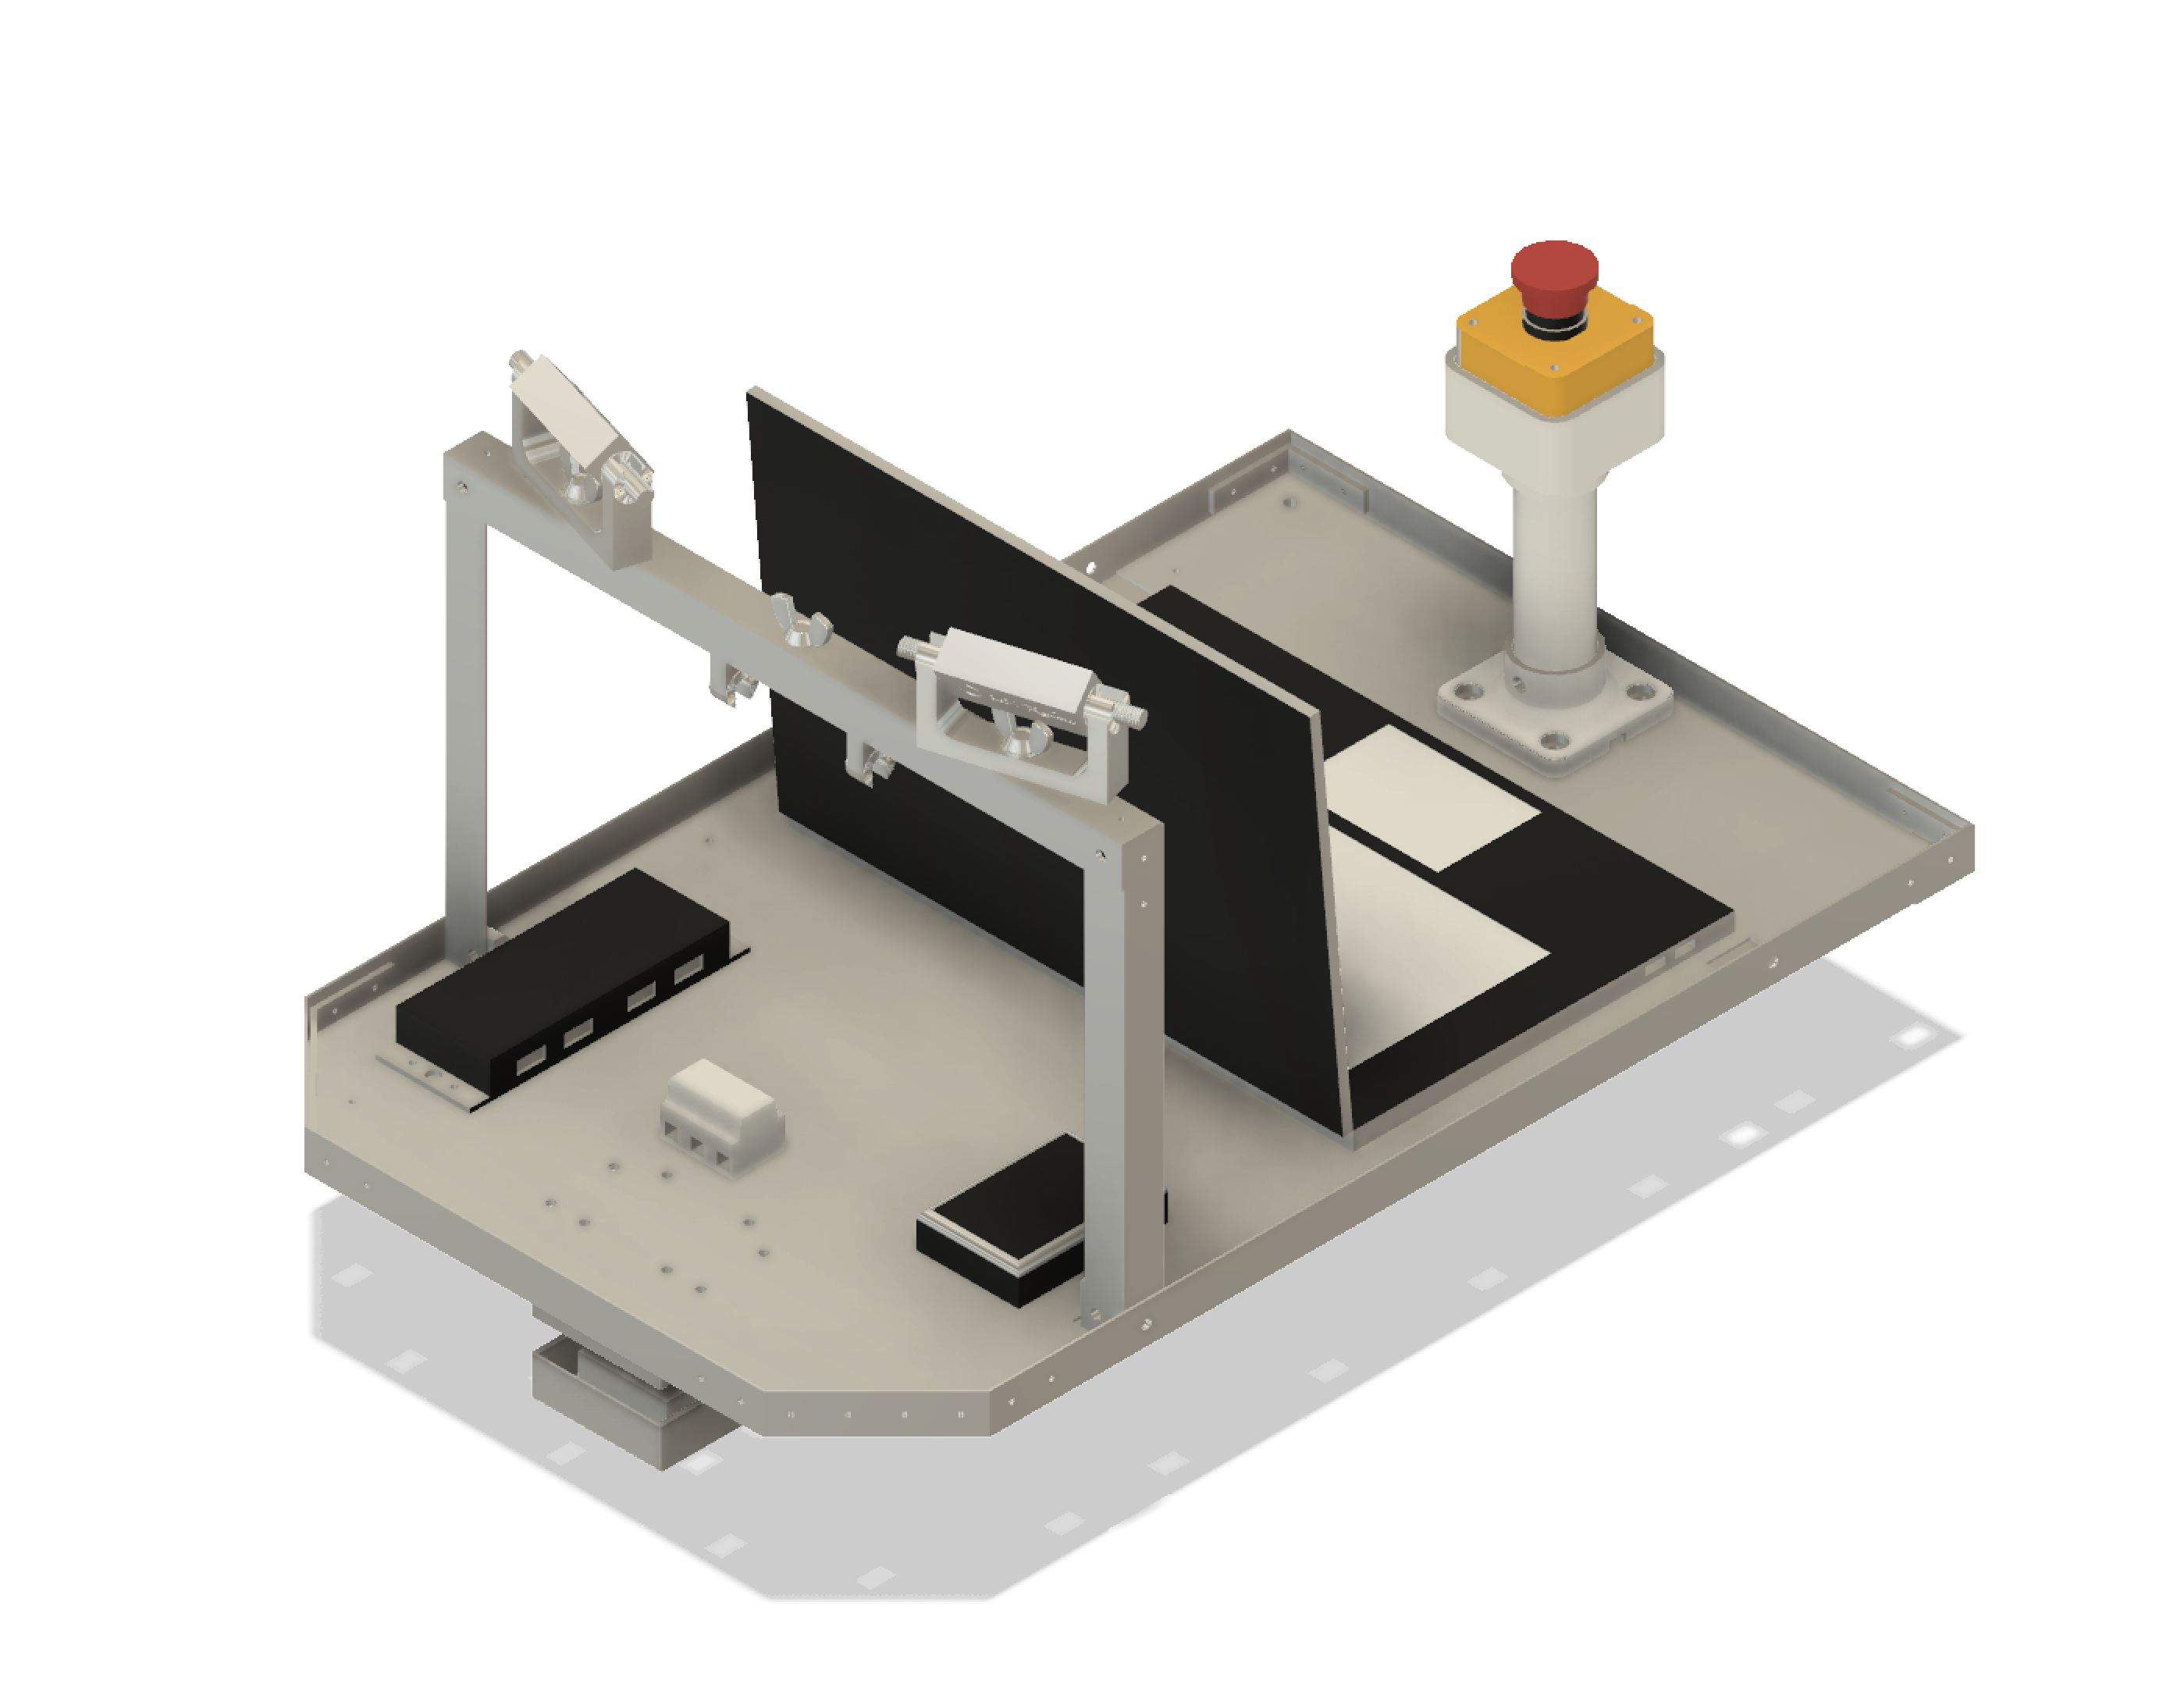
\includegraphics[width=0.9\columnwidth]{2018DesignMech.png}}
\caption{The Fusion CAD model of the body}
\label{Body1}
\end{figure}

\subsection{Wire Frame Superstructure}
The wire frame superstructure is the core component that bridges and secures other components. The wire frame is mainly made of aluminum materials. It is composed with three parts: a retrofit mounting system, a protective cage, and a camera rig. For retrofit mounting system, it is built with two aluminum clevis with two angle extrusions attached horizontally. The protective cage is made of aluminum in a trapezoid shape. The base cage can provide far enough strength to prevent the build plate away from any torsion or shear stresses from external forces or impacts. Similarly, the camera rig is also made of aluminum angle extrusions to provide a stable and flat platform for cameras. 

\subsection{Build Plate}
The main part of the build plate is a $\frac{1}{16} in.$ aluminum sheet, attached inside the protective cage securely. Since the build plate is entirely independent from the superstructure, it can be freely accessed and modified easily and independently without dissembling other structures. This can make the robot much easier to maintain and develop separately without complicated dis-assembly processes. On the bottom side of the plate, the lidar is also directly attached onto the sheet to remain protected and rigidly, while providing a clear detecting region. On the top side of the plate, hardware components such as a MCU (Micro Controller Unit) and a laptop can be safely mounted in place during the race.

\subsection{Other Mounting Components}
Other mounting components are mainly about the mounting system for mechanical E-Stop, and cameras. To keep the E-Stop in the required height and accessible area, a pillar with the combination of 3D printed mounting base and housing and an aluminum pipe was developed to elevate the E-Stop at the right height (as shown in Figure \ref{ESTOPMount}). In addition, the E-Stop pillar is installed right onto the wire frame superstructure to keep it securely and rigidly in place. For cameras, web cameras used in the previous competitions are kept to be used this year. To reduce the wobbliness of camera due to weak mounting mechanisms and sudden motion, a camera housing and mounting systems (as shown in Figure \ref{CameraMounts}) are designed in Fusion and 3D printed with ABS filaments. At the surface of each joint a rough triangle friction disk is designed to fix the camera while allowing the team able to freely adjust the camera angles to optimal positions. Camera mounts can then be placed onto the camera rig and fixed with bolts and nuts.

\begin{figure}[ht]
\centerline{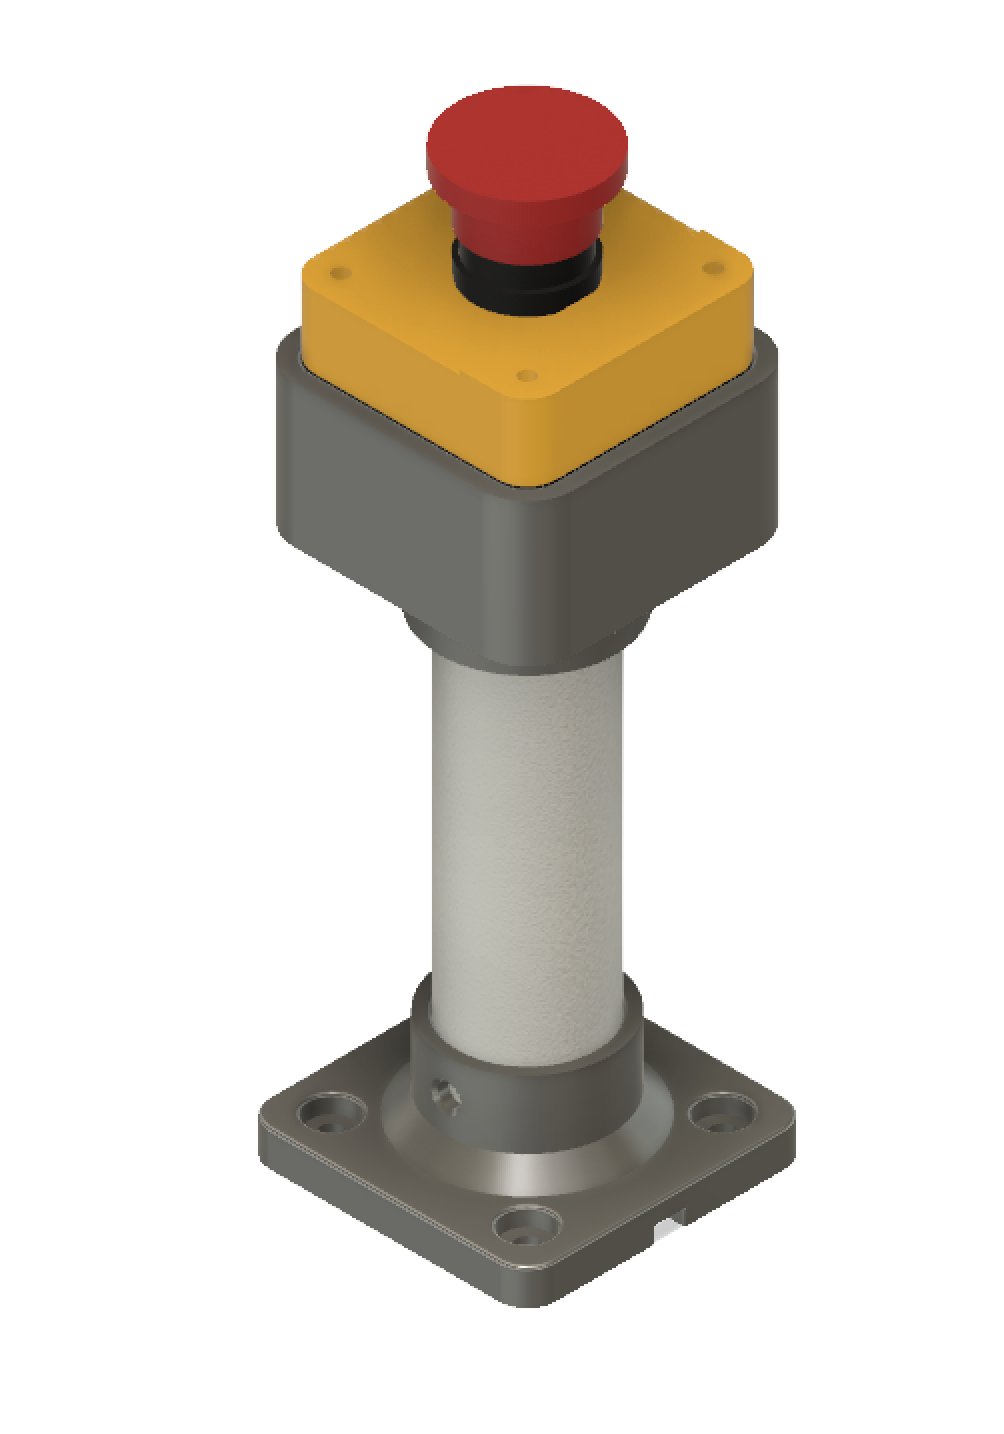
\includegraphics[width=0.5\columnwidth]{2018DesignMechESTOP.png}}
\caption{E-Stop mount in Fusion}
\label{ESTOPMount}
\end{figure}

\begin{figure}[ht]
\centerline{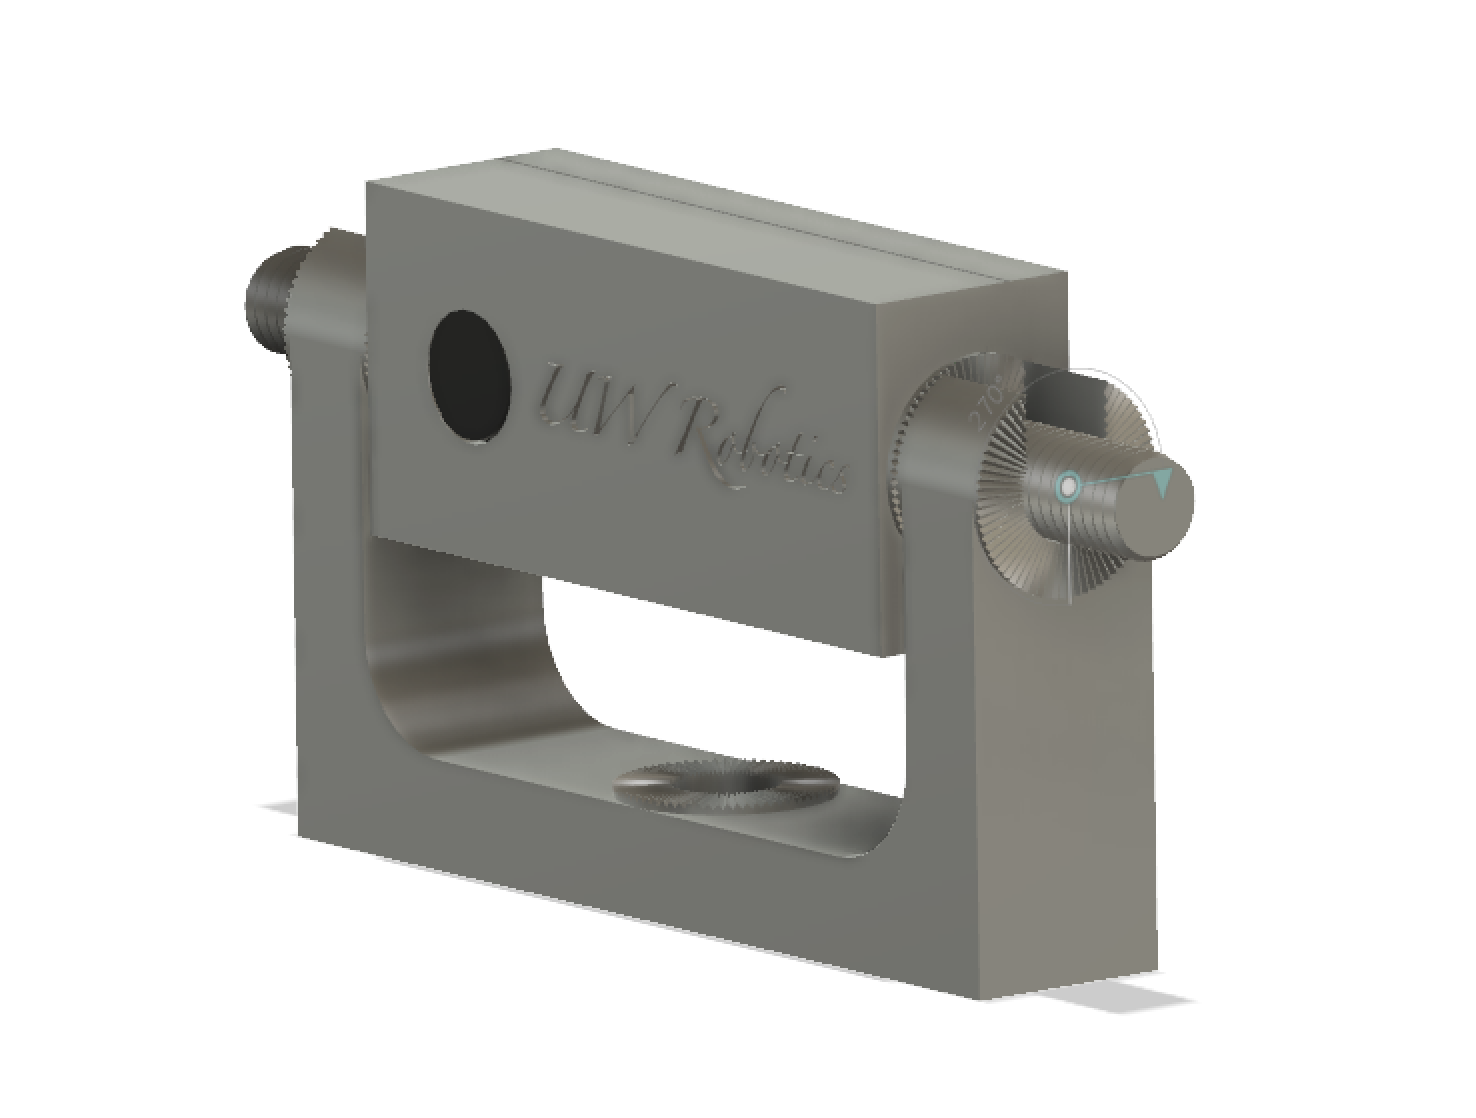
\includegraphics[width=0.5\columnwidth]{2018DesignMechCamMount.png}}
\caption{Camera mount in Fusion}
\label{CameraMounts}
\end{figure}

\section{Electrical Design}
The electrical design of the robot is based on the previous year’s design with new features introduced. The innovations in our electrical design can be categorized into sections including sensors, actuators, and the Arduino Shield.

\subsection{Power}
Two 12V 5800mAh Li-Po batteries, connected in series, provide the main 24V power rail to the robot. This 24V is directly used by the brush-less motor. To monitor the status of battery, a battery management system is integrated on the Arduino Shield. The system monitors the voltage of the battery and it relays thatto the main computer.

\subsection{Motor Controls}
The motors used for powering the vehicle comprise of two steering servos and one brush-less drive motor. The drive motor was controlled by a Castle Creations Electronic Speed Control unit (ESC). These motors are all controlled by the Arduino via PWM servo commands. In the event the Arduino PWM signal is neutral or missing, the ESC causes the drive motor to brake when powered.

\subsection{Sensors}
As described in the electrical design section, encoder counter is built from scratch using a 8-bit AVR MCU. The MCU which is programmed in low level C is capable to detect 512 encoder counts per revolution. The two encoder pulses are each detected as an external interrupt, and depending on the how the pulses change, the rotation direction and speed of the motor can be determined. The MCU communicates with the main Arduino via I2C, and returns the encoder count as unsigned 16 bit when the Arduino requests it. The calculation to convert from the encoder count to distance and speed is done on the Arduino side.
\begin{equation}
    V_{car} = \frac{d}{dt}(\frac{Count_{encoder}}{256})\cdot(R_{gear})\cdot(\pi D_{wheel})
\end{equation}
The Hokuyo 2D lidar provides the vehicle with range data for any obstacles within 30m, in a 270\degree plane in front of the vehicle.

The vision system comprises 3 cameras, two for line detection and one for traffic light detection. The occupancy grid is used to represent obstacles around the robot and this is created from a combination of the lidar data and camera data.

\section{Software Design}
The improvements over last year's software fall into three main categories: Architectural, Software development and testing, computer vision improvements and optimizations to sustaining higher speeds. These improvements allowed the team to radically improve our throughput and code quality while simultaneously increasing the performance of our robot.

\subsection{Software Development and Testing}
A holistic approach was taken to identify the limitations of the teams software development velocity. The main culprits were poor code documentation and lack of accessible testing.
To improve our code documentation the code base was completely refactored with a focus on clearer comments and aligning with a coherent coding style. This greatly improved readability and allowed new team members to get up to speed very quickly. To ensure that the new standards were carried forward, a code review was made compulsory before all code submissions.
To improve our software testing, there we're two major improvements made over the previous year. Firstly a simulation of the race and our competition vehicle were made. This simulation was developed using gazebo and ROS. The tracks were simulated to closely resemble the race environment with traffic cones and lane markings.
\begin{figure}[ht]
\centerline{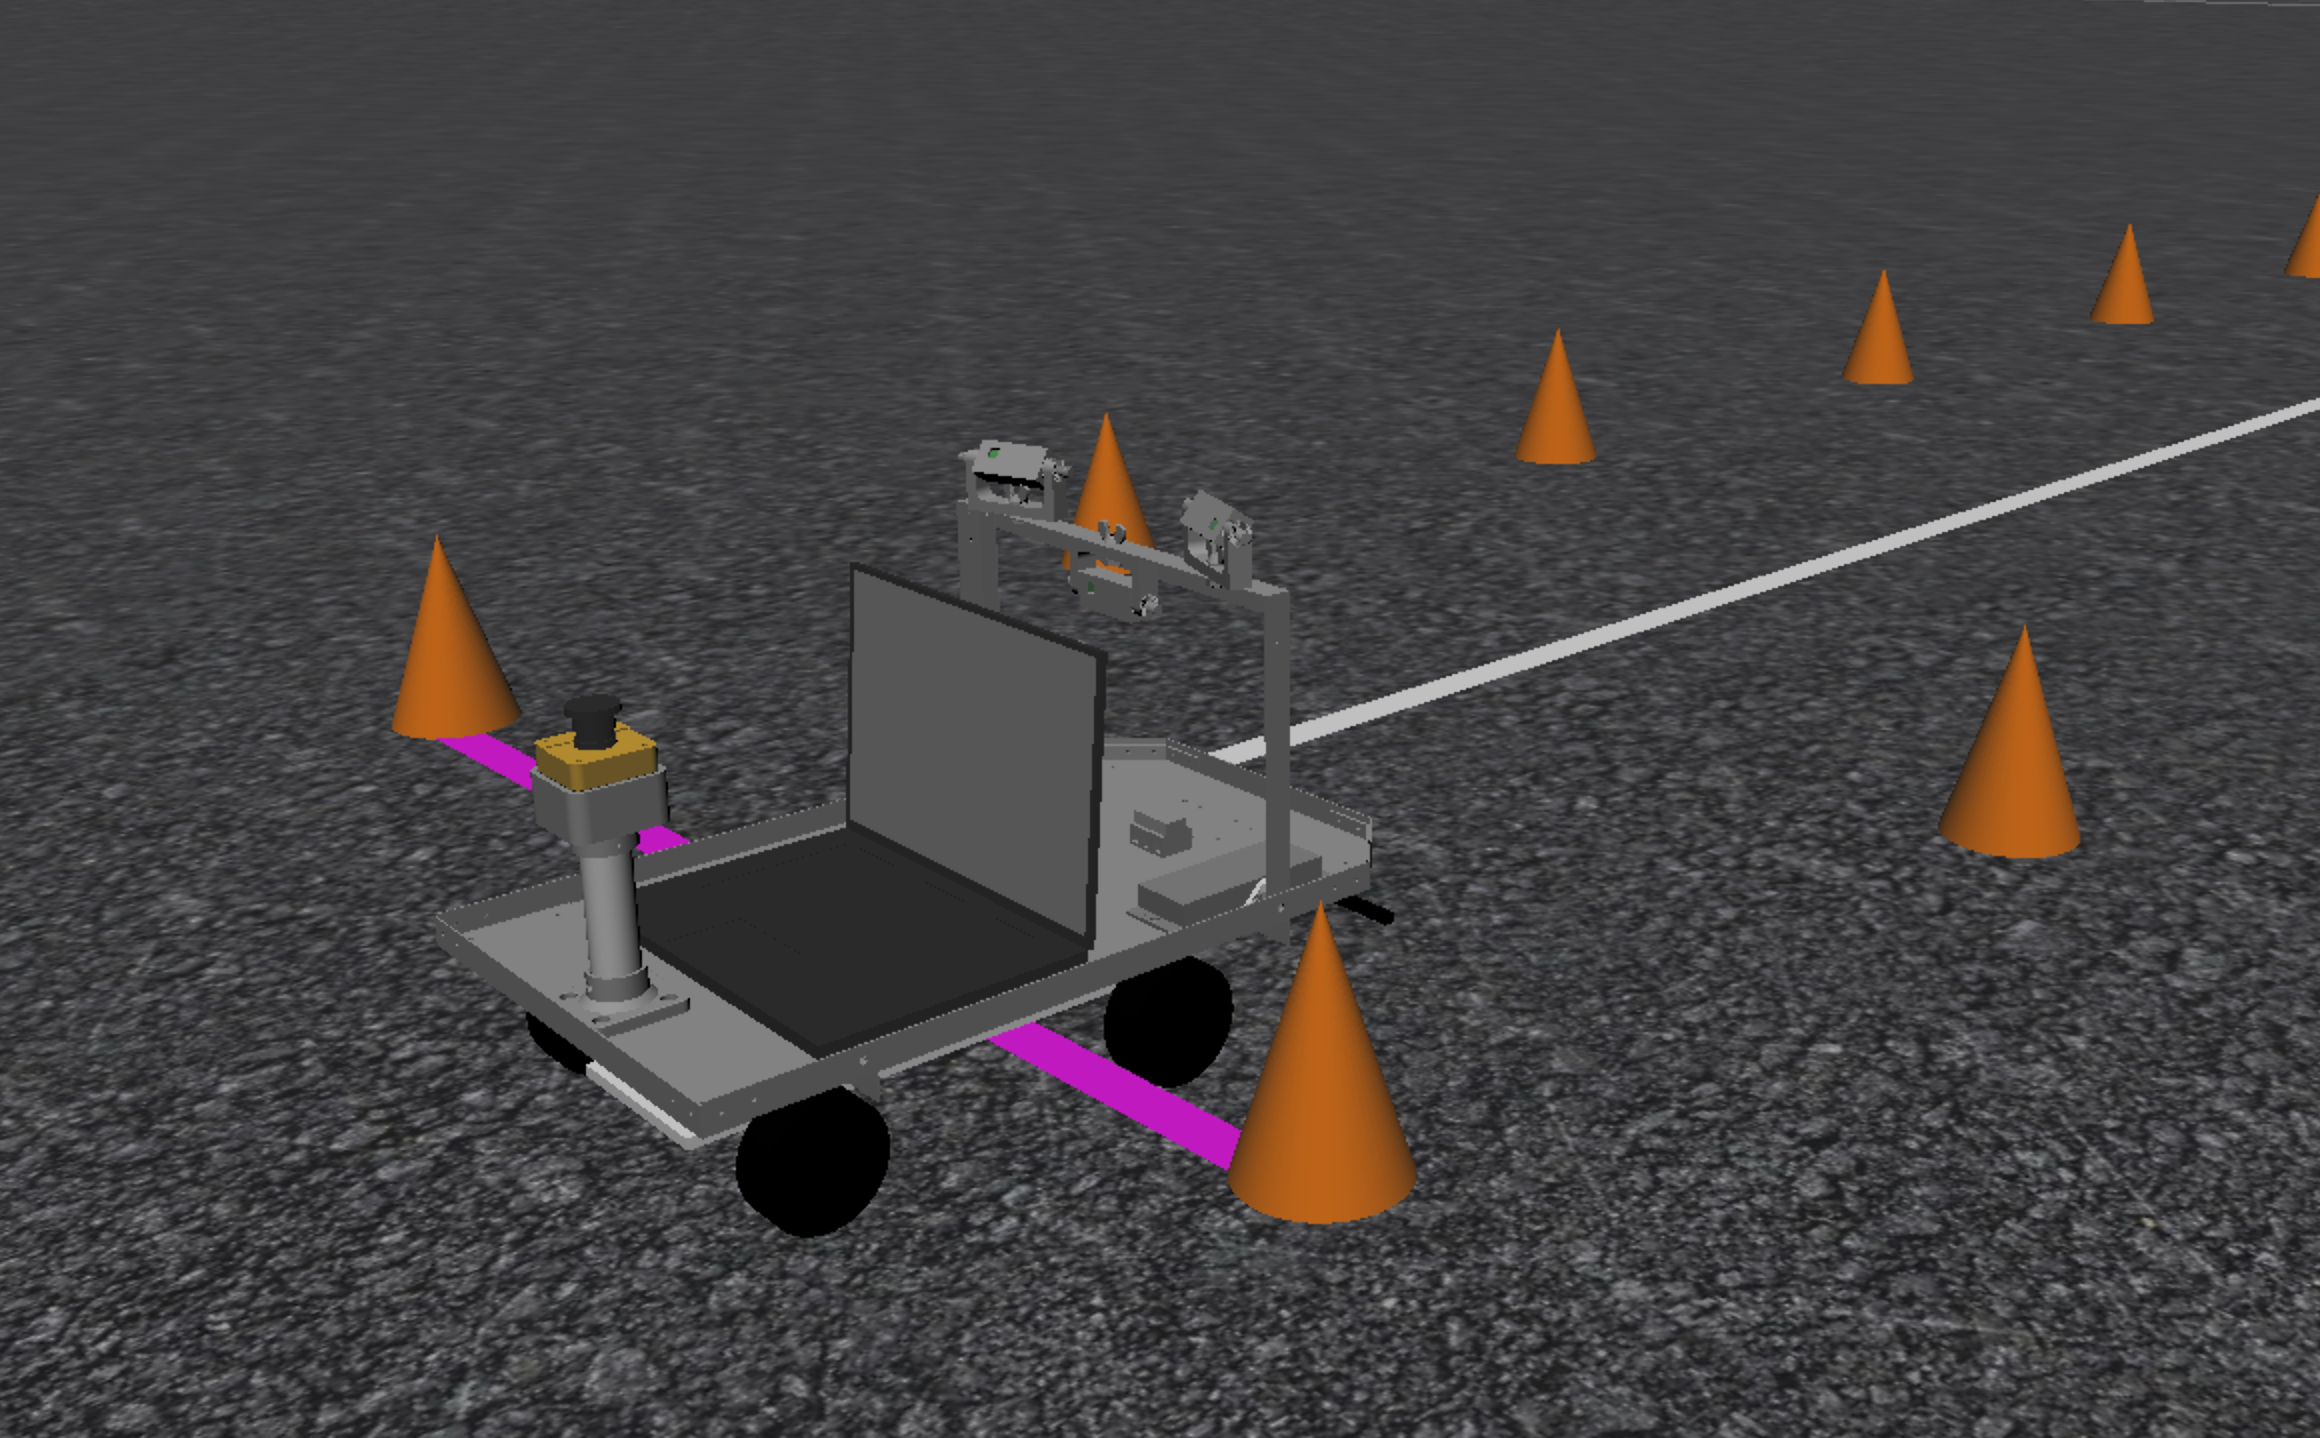
\includegraphics[width=0.9\columnwidth]{simulated_robot.png}}
\caption{Simulated Robot}
\label{Sim_Robot}
\end{figure}
The car was simulated with all the sensors currently on board the physical vehicle. The simulations allowed the software team to test both individual features and the entire system while the physical vehicle was still being built.

Secondly, we relied on recorded data from the past years competition to validate our code. A repository was created, containing the sensor data from previous competitions. This was used to validate our computer vision software and demonstrate it's superiority to software from the previous years.

\begin{figure*}[ht]
\centerline{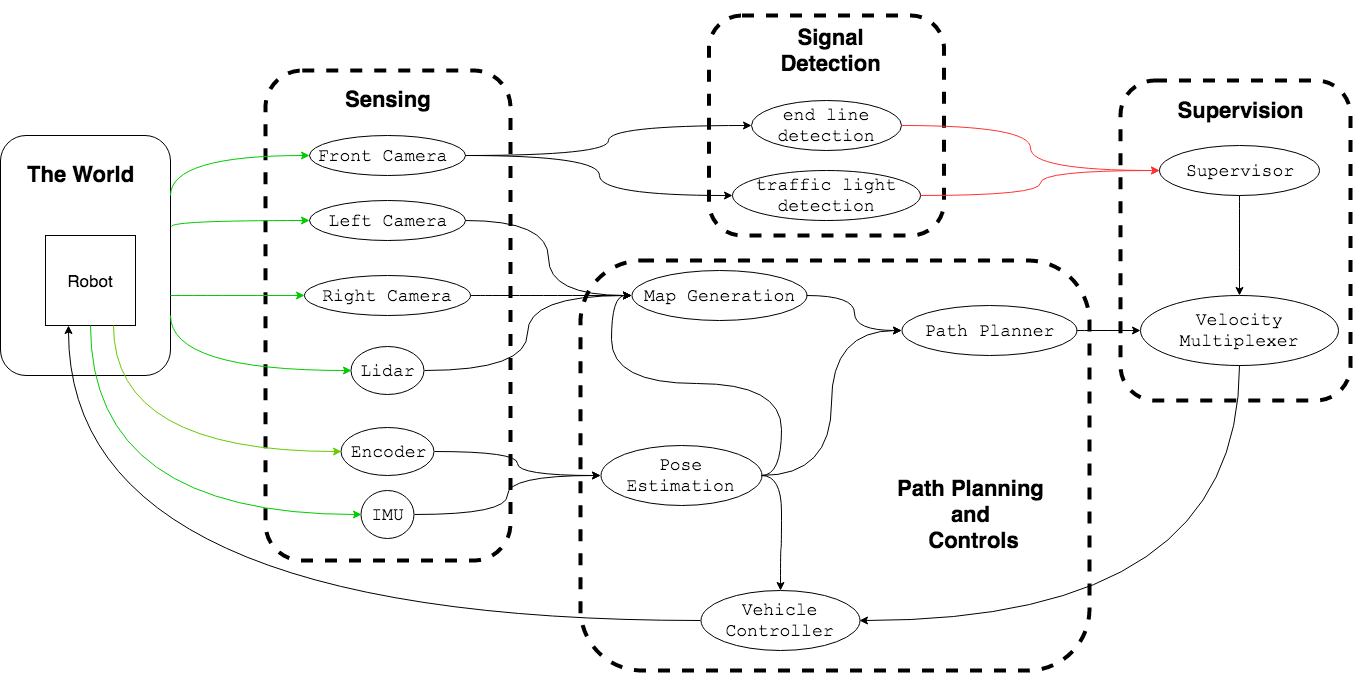
\includegraphics[width=2\columnwidth]{CodeStructure.png}}
\caption{The Software Architecture}
\label{Arch}
\end{figure*}
\subsection{Architectural}
In the previous structure each node was responsible for keeping track of the current state of the robot with no node responsible of keeping track of metrics or overseeing the operation of the vehicle. The new software architecture is illustrated below, with the addition of the supervisor node at the helm of the system. As seen in \ref{Arch}.

The sensing software consists of device drivers and ROS nodes that publish sensor data to other nodes to be consumed. Most of the software in this section is provided by vendors or the open source community.
The path planning and controls sections are responsible for determining where to go and keeping the car on that path.
The signal detection section consists of ROS nodes responsible for detecting important signals like a traffic light changes and the line signifying the end of the race. They communicate these events to the supervisor which then decides on the course of action.
The supervisor node is a module designed to manage high level decisions and keep track of useful race metrics. It provides an interface for signal detection nodes to indicate that an event has occurred. Using it's knowledge of the current state of the robot, it decides when to start and stop the car.
The supervisor node also keeps track of some useful variables; namely the race type, start and end times, lap count, average speed, and battery life. When the race is finished, a few of these variables are stored and saved into a text file. The race is started when a traffic light signal is received, and is ended when either the lap count is reached for that race, which is incremented by an end line detection signal, or if the battery life dips below 10%.

\subsection{Computer Vision}
This competition year, huge strides were made in improving the robustness and functionality of our computer vision software. To improve the robustness of our lane detection system a shadow removal algorithm was added as a pre-processing step on each of our cameras. To improve our traffic light detection in all conditions a machine learning classifier was added to help detect traffic lights in images. End line detection was improved considerably over past years as well, largely due to the addition of a new hysteresis filter on the camera stream. 

\subsubsection{Shadow Removal}
In last year's competition, the robot had difficulty in reliably tracking lane lines under variable lighting conditions, such as when buildings or robots cast shadows onto the track. As a result, this year's team implemented a shadow detection and removal pre-processing step, based on work done by Murali et al. \cite{ShadRemoval} in order to address this issue.
First, to detect shadows, the algorithm calculates the mean value of each plane in the Lab colour space and applies a threshold on the L and b values. The Lab colour space was designed to be uniform with respect to human vision, so it could better model visually perceived changes, such as variations in lightness that would indicate a shadow region. An example is shown in Figure ~\ref{Shadow1}.
\begin{figure}[ht]
\centerline{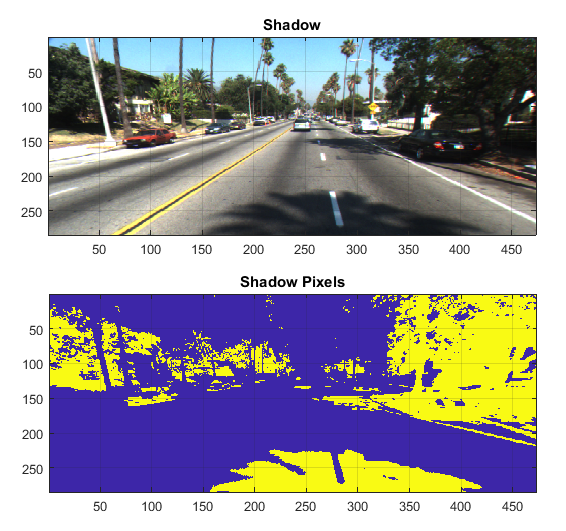
\includegraphics[width=0.9\columnwidth]{X1.png}}
\caption{Shadow Detection Using Lab Colour Space}
\label{Shadow1}
\end{figure}

To prepare for shadow removal, the shadow mask is dilated – to smooth out holes and sharp edges – and then separated into shadow regions. For each shadow region, the algorithm calculates the ratio of red, green, and blue values between the area inside the mask and the area just outside the mask. To remove shadows, the shadow region's RGB values are multiplied by these ratios.

The last, and slowest, step is to correct for over-illuminated edges in the shadow regions, since the outer edges of shadows tend to be brighter than the inner region. To do this, a median filter is applied on the edges of each shadow region.

There were two issues the team encountered with this shadow detection and removal approach. The first was that the over-illumination correction took the most time to run, but often blurred out lane lines through its median filter, especially if the shadow was spotty and had edges in its interior. However, the team did not expect to encounter this situation in competition and the resulting images were often more useful for line tracking than the originals. An alternative method to correct for over-illumination could be considered in the future. Second, since the shadow detection relies on a mean value for the lightness (L) over the entire image, a frame with extreme highlights can cause the algorithm to misidentify shadows and over-illuminate entire regions. Again, this was not expected to be seen in competition since this issue was most common with a blown-out sky region and the robot's cameras are directed towards the ground.

Figure ~\ref{Shadow6} displays the final result, showing the lane detection before and after the shadow removal pre-processing step for a test image.

\begin{figure}[ht]
\centerline{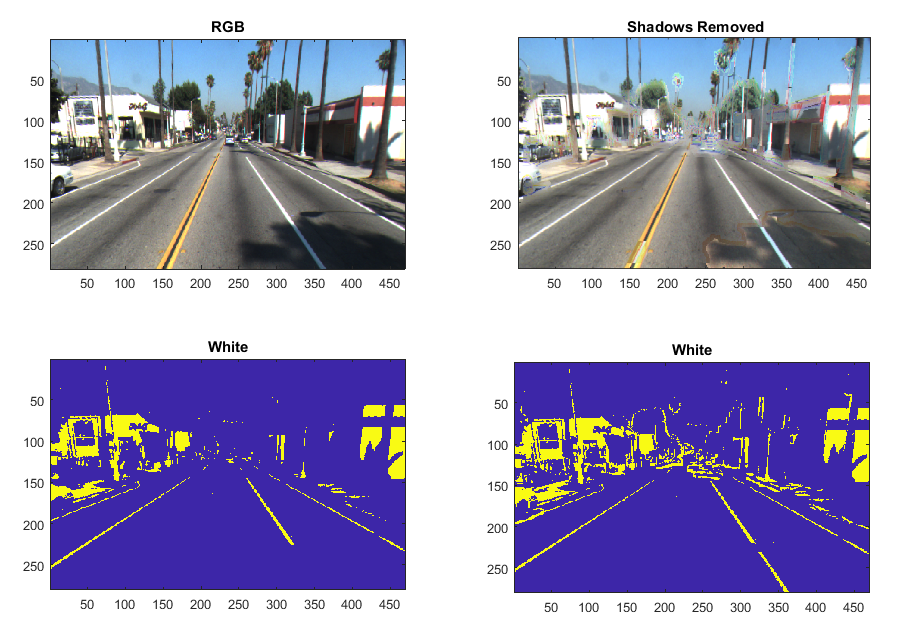
\includegraphics[width=0.9\columnwidth]{X6.png}}
\caption{White Line Detection Before and After Shadow Removal}
\label{Shadow6}
\end{figure}

\subsubsection{Traffic Light Detection}
The traffic light detection process is initiated starting with availability of image data supplied by the camera sensors, which is relayed in the form of a mutable message data structure to the system nodes. Detection of the traffic light object is performed using YOLO (“You Only Look Once”)\cite{TrafLight}, a neural net based object classifier which is integrated as a separate system node responsible for identifying and outlining the location of specific objects within an given image \ref{TrafficLight}. As an example, Figure 1.0 shows YOLO detecting a traffic light object from camera image.
\begin{figure}[ht]
\centerline{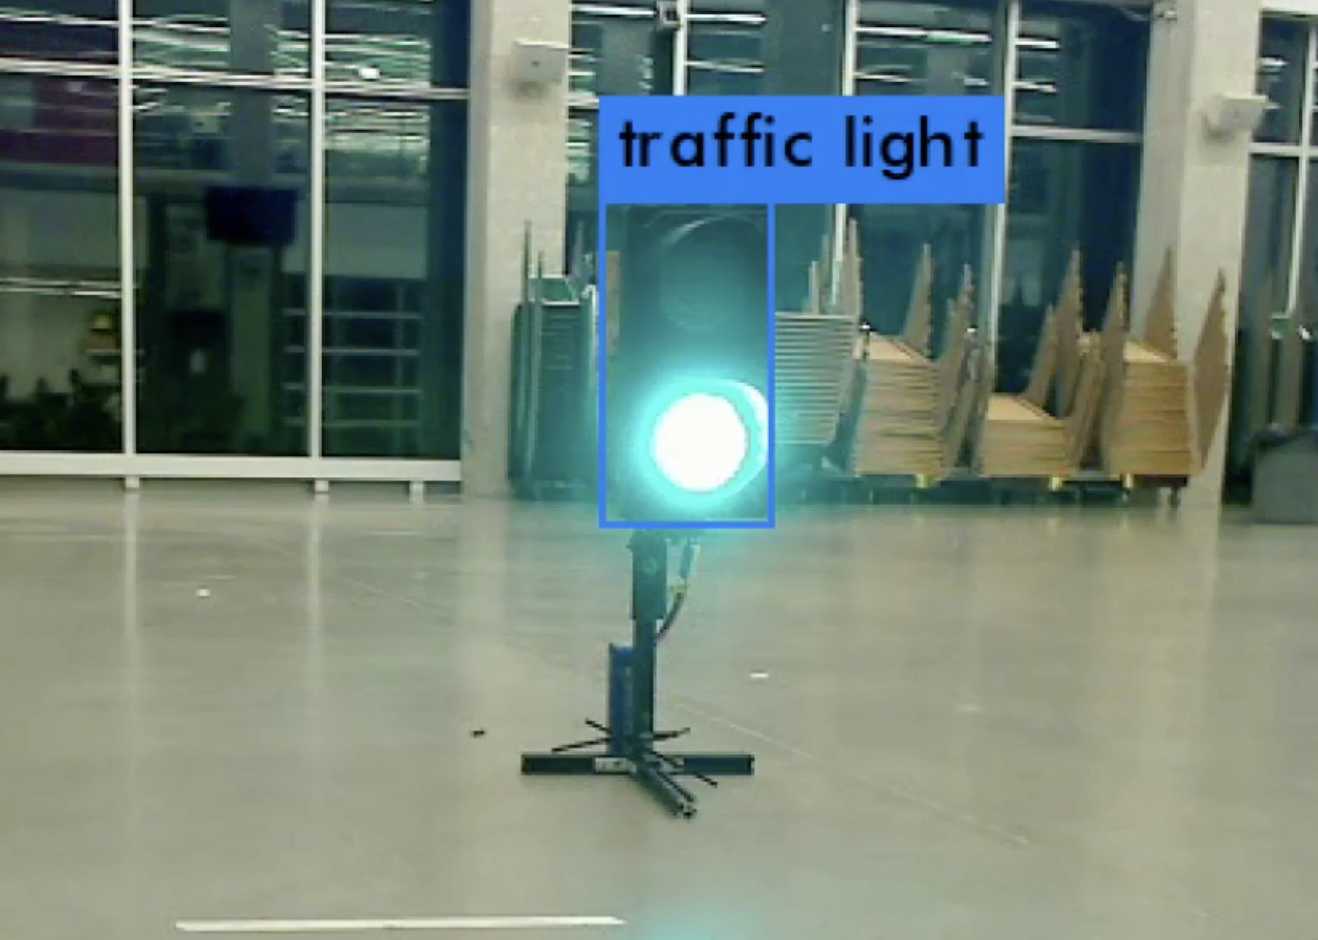
\includegraphics[width=0.9\columnwidth]{traffic_green.png}}
\caption{White Line Detection Before and After Shadow Removal}
\label{TrafficLight}
\end{figure}

Once a traffic light object is detected, the camera image is cropped to the bounding box of the traffic light, which is then sent over to the traffic light processor node. Within this section of the system, the image, existing in RGB color space is converted into a hue, value, saturation (HSV) space. Gaussian blur is also applied to the image to smooth out irregularities and remove noise to increase analysis accuracy. The state of the traffic light is detected by applying a filter that isolates pixels that correspond to a certain color range to distinguish red and green colors in a diverse set of lighting conditions. The traffic light color state is determined based on of the prominence in either color value. Upon detection of a green traffic light, a service call is invoked, signalling the start of the race. This was able to detect traffic lights in 93\% of the time in contrast to our previous algorithm which only worked on 75\% of samples provided.

\subsubsection{End line Detection}
To detect the end line, the image is converted to the HSV color-space and filtered for Magenta. A Gaussian blur is then performed on the image to reduce small detection errors. Finally, blob detection is used to filter for minimum area and non-circularity. This detection algorithm is inserted between a hysteresis counter procedure, that increments when detection is true and decrements when detection is false. This prevents false positive detection of the algorithm. Once complete a service call is invoked signalling the completion of a lap.

\subsection{Path Planning and Controls}
The path planning framework was overhauled from the previous year. Whereas last year's path planner was entirely reactive, the new path planner incorporates a look ahead distance whenever lane markings are present. It uses these lane markings to pick a point ahead in space to plan a path to, this helps it sustain higher speeds for longer stretches of time. The path is continually reassessed and planned and a fairly low frequency of 1 Hz. If any obstacles are detected along the path closer than a certain threshold the path planner falls back to the trajectory roll-out algorithm which can run at a much higher frequency of up to 20Hz.
To remain on the path that was selected the robot utilizes an MPC. This is updated with the robots estimate of its current position by a sensor fusion ROS node. The MPC computes the error between where the robot is and where it should be, often referred to as the cross track error and generates steering and throttle commands to follow the path.

\subsubsection{Medium Range Planning}
To plan a feasible path to a position farther ahead an RRT planner is employed. When provided a point along the track farther ahead of it. The planner takes the kinematic model into account and generates an obstacle free path for the robot to follow.

\subsubsection{Close Range Obstacle Avoidance}
The trajectory rollout algorithm from previous year is preserved and it is responsible for engaging in close range evasive maneuvers when unforeseen obstacles arise. These obstacles could be other cars on the track or humans that might cross the track.

\subsubsection{Sensor Fusion and Controls}
The velocity information from the encoder and orientation and acceleration information from IMU were fused together using an Extended Kalman Filter to provide the path planner with the vehicles pose. The MPC uses the vehicle pose and the generated path to generate steering and throttle commands for the robot. The MPC is superior to our previous sole PID controller because it computes commands with a knowledge of the kinematics of the vehicle.

\section{Conclusion}
Thus far, the success of the current design can only be assessed relative to the performance of the previous vehicle. Many weak points were addressed, and significant performance improvements were made. The body was redesigned to be more durable, repairable  and serviceable. The traffic light detection strategy was made much more robust, and has been tested successfully in varied environments. The path planner was improved to enable sustained high speed driving and retain vehicle responsiveness. The teams software development practices were updated and enforced.

% if have a single appendix:
%\appendix[Proof of the Zonklar Equations]
% or
%\appendix  % for no appendix heading
% do not use \section anymore after \appendix, only \section*
% is possibly needed

% use appendices with more than one appendix
% then use \section to start each appendix
% you must declare a \section before using any
% \subsection or using \label (\appendices by itself
% starts a section numbered zero.)
%


% use section* for acknowledgement
\section*{Acknowledgment}

The authors would like to thank members of the WAVE lab who provided hardware used on the robot. They would also like to thank Matthew Post for his mentorship and continued support of the team.

Additional note - All work done on changes to mechanical, electrical and software design was performed by team members who had no former experience with the competition, while returning members took on a mentoring role. The new members should be especially noted for their dedication, work ethic and ingenuity. They made this happen.

% Can use something like this to put references on a page
% by themselves when using endfloat and the captionsoff option.
\ifCLASSOPTIONcaptionsoff
  \newpage
\fi



% trigger a \newpage just before the given reference
% number - used to balance the columns on the last page
% adjust value as needed - may need to be readjusted if
% the document is modified later
%\IEEEtriggeratref{8}
% The "triggered" command can be changed if desired:
%\IEEEtriggercmd{\enlargethispage{-5in}}

% references section

% can use a bibliography generated by BibTeX as a .bbl file
% BibTeX documentation can be easily obtained at:
% http://www.ctan.org/tex-archive/biblio/bibtex/contrib/doc/
% The IEEEtran BibTeX style support page is at:
% http://www.michaelshell.org/tex/ieeetran/bibtex/
%\bibliographystyle{IEEEtran}
% argument is your BibTeX string definitions and bibliography database(s)
%\bibliography{IEEEabrv,../bib/paper}
%
% <OR> manually copy in the resultant .bbl file
% set second argument of \begin to the number of references
% (used to reserve space for the reference number labels box)
\begin{thebibliography}{2}

\bibitem{TrafLight}
J. Redmond, R. Girshick, A. Farhadi, and S. Divvala, \emph{You Only Look Once: Unified, Real-Time Object Detection}. Washington, tech, 2015

\bibitem{ShadRemoval}
Murali, Saritha and V K, Govindan. \emph{Shadow Detection and Removal from a Single Image Using LAB Color Space}. Cybernetics and Information Technologies, 2013. 
\end{thebibliography}

% biography section
% 
% If you have an EPS/PDF photo (graphicx package needed) extra braces are
% needed around the contents of the optional argument to biography to prevent
% the LaTeX parser from getting confused when it sees the complicated
% \includegraphics command within an optional argument. (You could create
% your own custom macro containing the \includegraphics command to make things
% simpler here.)
%\begin{biography}[{\includegraphics[width=1in,height=1.25in,clip,keepaspectratio]{mshell}}]{Michael Shell}
% or if you just want to reserve a space for a photo:

%\begin{IEEEbiography}[{\includegraphics[width=1in,height=1.25in,clip,keepaspectratio%]{picture}}]{John Doe}
%\blindtext
%\end{IEEEbiography}

% You can push biographies down or up by placing
% a \vfill before or after them. The appropriate
% use of \vfill depends on what kind of text is
% on the last page and whether or not the columns
% are being equalized.

%\vfill

% Can be used to pull up biographies so that the bottom of the last one
% is flush with the other column.
%\enlargethispage{-5in}

% that's all folks
\end{document}
